\documentclass[tikz,border=8pt]{standalone}
% Shared look for every TikZ diagram. Load with \input{../../tools/tikz-style.tex}
\usepackage[T1]{fontenc}
\usepackage{lmodern}
\renewcommand{\sfdefault}{lmr}  % diagrams use the same serif as the text
\usetikzlibrary{arrows.meta, positioning, shapes.geometric, calc, fit, backgrounds}
\definecolor{cblue}{HTML}{4C78A8}
\definecolor{corange}{HTML}{F58518}
\definecolor{cgreen}{HTML}{54A24B}
\definecolor{cred}{HTML}{E45756}
\definecolor{cpurple}{HTML}{B279A2}
\definecolor{cgrey}{HTML}{6B6B6B}
\tikzset{
  every picture/.style={font=\sffamily, line width=1.2pt},
  box/.style={draw=#1, fill=#1!12, rounded corners=4pt, align=center, inner sep=7pt, minimum height=1.1cm},
  box/.default=cgrey,
  arrow/.style={-{Stealth[length=3mm]}, draw=cgrey, line width=1.4pt},
  title/.style={font=\sffamily\bfseries\Large},
  note/.style={font=\sffamily\small, text=cgrey, align=center},
}
\AtBeginDocument{\hyphenpenalty=10000 \exhyphenpenalty=10000}

\begin{document}
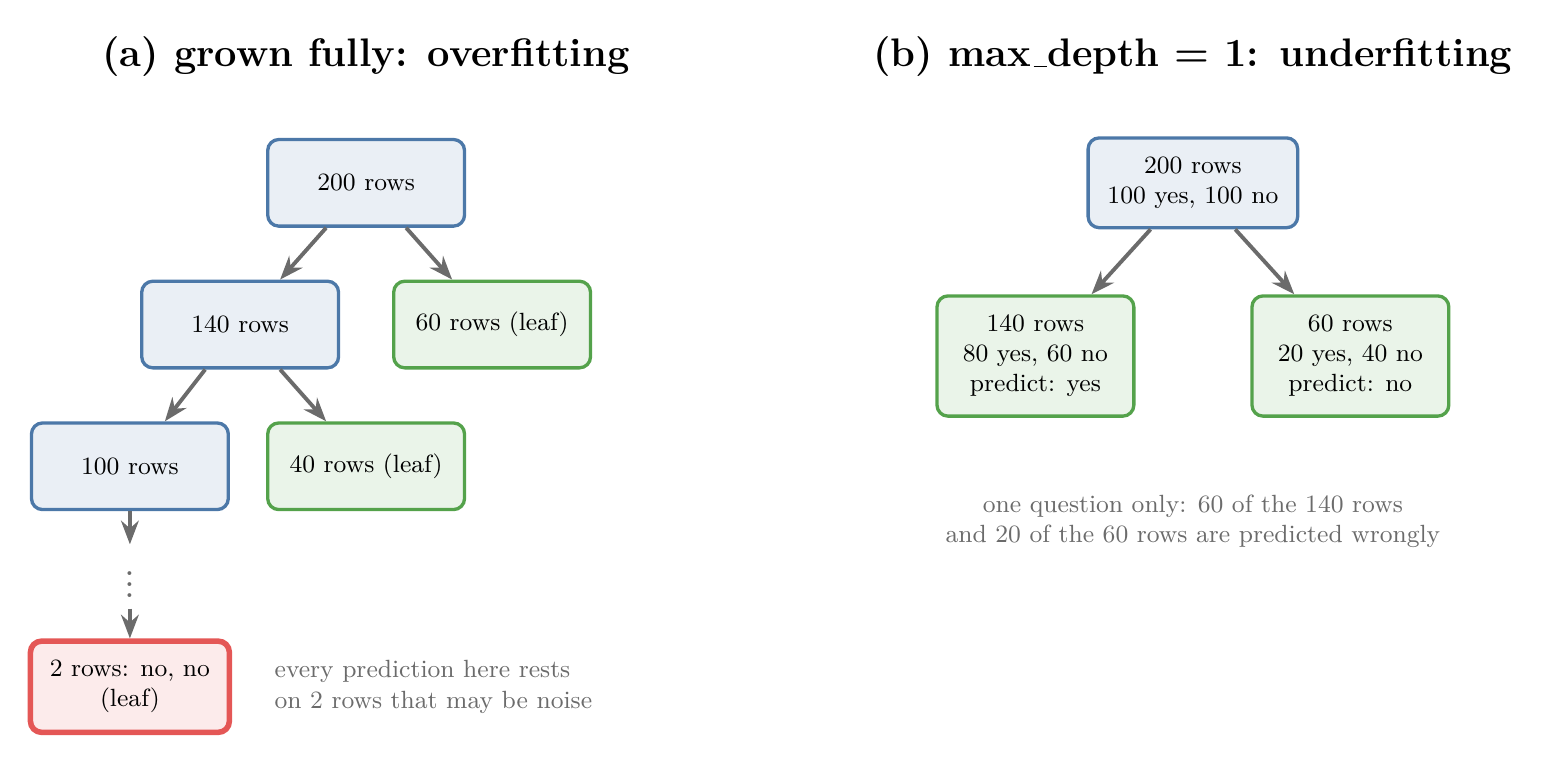
\begin{tikzpicture}[
  n/.style={box=cblue, minimum width=2.5cm, font=\sffamily\small},
  lf/.style={box=cgreen, minimum width=2.5cm, font=\sffamily\small},
  bad/.style={box=cred, minimum width=2.5cm, font=\sffamily\small, line width=2pt}]
  % (a) overfitting
  \node[title] at (0,1.6) {(a) grown fully: overfitting};
  \node[n] (a0) at (0,0) {200 rows};
  \node[n] (a1) at (-1.6,-1.8) {140 rows};
  \node[lf] (a2) at (1.6,-1.8) {60 rows (leaf)};
  \node[n] (a3) at (-3.0,-3.6) {100 rows};
  \node[lf] (a4) at (0,-3.6) {40 rows (leaf)};
  \node[cgrey, font=\sffamily\Large] (a5) at (-3.0,-5.0) {$\vdots$};
  \node[bad] (a6) at (-3.0,-6.4) {2 rows: no, no\\(leaf)};
  \draw[arrow] (a0) -- (a1); \draw[arrow] (a0) -- (a2);
  \draw[arrow] (a1) -- (a3); \draw[arrow] (a1) -- (a4);
  \draw[arrow] (a3) -- (a5); \draw[arrow] (a5) -- (a6);
  \node[note, anchor=west, align=left] at (-1.3,-6.4) {every prediction here rests\\on 2 rows that may be noise};
  % (b) underfitting
  \begin{scope}[xshift=10.5cm]
  \node[title] at (0,1.6) {(b) max\_depth = 1: underfitting};
  \node[n] (b0) at (0,0) {200 rows\\100 yes, 100 no};
  \node[lf] (b1) at (-2,-2.2) {140 rows\\80 yes, 60 no\\predict: yes};
  \node[lf] (b2) at (2,-2.2) {60 rows\\20 yes, 40 no\\predict: no};
  \draw[arrow] (b0) -- (b1); \draw[arrow] (b0) -- (b2);
  \node[note, align=center] at (0,-4.3) {one question only: 60 of the 140 rows\\and 20 of the 60 rows are predicted wrongly};
  \end{scope}
\end{tikzpicture}
\end{document}
